% !TEX root =  ../main_manuscript.tex 
\subsection{Statistical Model}
For developing an upgrading-risk prediction model, the data we utilized from the PRIAS cohort was patient age at inclusion in AS, longitudinally measured PSA, timing of repeat biopsies and Gleason grades, and observed time of upgrading. Analysis of this data required modeling the within-patient correlation for PSA, the association between the Gleason grades and PSA profiles of a patient, and handling missing PSA measurements after a patient experienced upgrading. In such situations, a commonly used model is the joint model for time-to-event and longitudinal data~\citep{tomer2019,coley2017prediction,rizopoulos2012joint}.

Our joint model consisted of two sub-models. First, a linear mixed sub-model~\citep{laird1982random} for longitudinally measured PSA (log-transformed). Second, a relative-risk sub-model (similar to the Cox model) for obtaining the cause-specific upgrading-risk. We included patient age in both sub-models. In the PSA sub-model, we fitted a unique curve to the PSA measurements of each patient (Panel~A, Figure~\ref{fig:jmExplanationPlot_113}). Subsequently, we calculated the mathematical derivative of the patient's fitted PSA profile (Equation~2, Supplementary~A), to obtain his follow-up time specific instantaneous PSA velocity (Panel~B, Figure~\ref{fig:jmExplanationPlot_113}). This instantaneous velocity is a stronger predictor of upgrading than the widely used average PSA velocity~\citep{cooperberg2018refined}. We modeled the impact of PSA on upgrading-risk by employing fitted PSA value and instantaneous velocity as predictors in the risk sub-model. Also, we included the time of the latest negative biopsy in the risk sub-model (Panel~C, Figure~\ref{fig:jmExplanationPlot_113}). The parameters of the two sub-models were estimated jointly (Supplementary~A) using the R package \textbf{JMbayes}~\citep{rizopoulosJMbayes}. 

\begin{figure}
\centerline{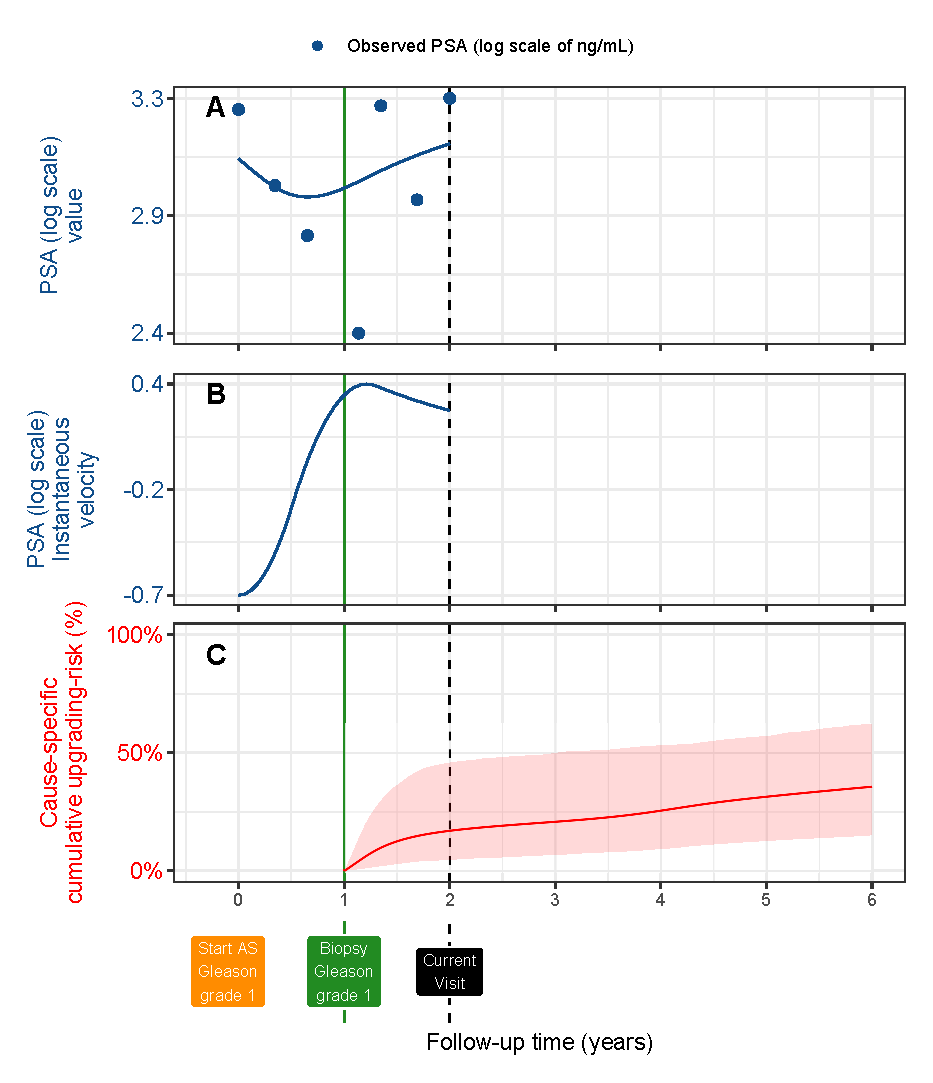
\includegraphics[width=\columnwidth]{images/jmExplanationPlot_113.eps}}
\caption{\textbf{Illustration of the joint model on a real PRIAS patient}. \textbf{Panel~A:} Observed PSA (blue dots) and fitted PSA (solid blue line), log-transformed from ng/mL. \textbf{Panel~B:} Estimated instantaneous velocity of PSA (log-transformed). \textbf{Panel~C}: Predicted cause-specific cumulative upgrading-risk (95\% credible interval shaded). Upgrading is defined as an increase in the Gleason grade group from group~1~\citep{epsteinGG2014} to 2 or higher. This upgrading-risk is calculated starting from the time of the latest negative biopsy (vertical green line at year one of follow-up). The joint model estimated it by combining the fitted PSA (log scale) value and instantaneous velocity, and time of the latest negative biopsy. Black dashed line at year two denotes the time of current visit.}
\label{fig:jmExplanationPlot_113}
\end{figure}

\subsection{Risk Prediction and Model Validation}
Our model provides predictions for upgrading-risk over the entire future follow-up period of a patient. Predictions also automatically update over follow-up as more patient data becomes available (Figure~5, Supplementary~B). We validated our PRIAS based model internally in the PRIAS cohort, and externally in the largest six GAP3 database cohorts. We employed calibration plots~\citep{royston2013external,steyerberg2010assessing} and follow-up \textit{time-dependent} mean absolute risk prediction error or MAPE~\citep{rizopoulos2017dynamic} to graphically and quantitatively evaluate our model's risk prediction accuracy, respectively. We assessed our model's ability to discriminate between patients who experience/do not experience upgrading via the time-dependent area under the receiver operating characteristic curve or AUC~\citep{rizopoulos2017dynamic}. 

The aforementioned \textit{time-dependent} AUC and MAPE~\citep{rizopoulos2017dynamic} are temporal extensions of their standard versions~\citep{steyerberg2010assessing} in a longitudinal setting. Specifically, at every six months of follow-up, we calculated a unique AUC and MAPE for predicting upgrading-risk in the subsequent one year (Supplementary~B.1). For emulating a realistic situation, we calculated the AUC and MAPE at each follow-up using only the validation data available until that follow-up. Last, to resolve any potential model miscalibration in validation cohorts, we aimed to recalibrate our model's baseline hazard of upgrading (Supplementary~B.1), individually for each cohort.